\documentclass[submission,copyright,creativecommons]{eptcs}
\providecommand{\event}{LFMTP 2022} % Name of the event you are submitting to
%\usepackage{breakurl}             % Not needed if you use pdflatex only.
\usepackage{underscore}           % Only needed if you use pdflatex.

\title{An Implementation of Set Theory with Pointed Graphs in Dedukti}
\author{Valentin Blot
\institute{Inria, France\\
LMF, ENS Paris-Saclay, France}
\email{valentin.blot@inria.fr}
\and
Gilles Dowek
\institute{Inria, France\\
LMF, ENS Paris-Saclay, France}
\email{gilles.dowek@ens-paris-saclay.fr}
\and
Thomas Traversié
\institute{CentraleSupélec, France}
\email{thomas.traversie@inria.fr}
}

\def\titlerunning{An Implementation of Set Theory with Pointed Graphs in Dedukti}
\def\authorrunning{V. Blot, G. Dowek, T. Traversié}

%% My packages

\usepackage{tikz}
\usepackage{url}
\usepackage[utf8]{inputenc}
\usepackage[T1]{fontenc}

%% Lambdapi code

\usepackage{listings}
\usepackage{amssymb}
\usepackage{mathtools}
\usepackage{xcolor}
\definecolor{green}{RGB}{0,130,0}
\definecolor{lightgrey}{RGB}{240,240,240}

\lstdefinelanguage{Lambdapi}
{
  inputencoding=utf8,
  extendedchars=true,
  numbers=none,
  numberstyle={},
  tabsize=2,
  basicstyle={\ttfamily\upshape\mdseries},
  backgroundcolor=\color{lightgrey},
  keywords={abort,admit,admitted,apply,as,assert,assertnot,associative,assume,begin,builtin,commutative,compute,constant,debug,end,fail,flag,focus,generalize,have,in,induction,inductive,infix,injective,left,let,notation,off,on,opaque,open,prefix,print,private,proofterm,protected,prover,prover_timeout,quantifier,refine,reflexivity,require,rewrite,right,rule,sequential,simplify,solve,symbol,symmetry,type,TYPE,unif_rule,verbose,why3,with},
  sensitive=true,
  keywordstyle=\color{blue},
  morecomment=[l]{//},
  commentstyle={\itshape\color{red}},
  string=[b]{"},
  stringstyle=\color{orange},
  showstringspaces=false,
  literate=
  {↪}{$\hookrightarrow$}1
  {→}{$\rightarrow$}1
  {Π}{$\Pi$}1
  {≔}{\quad $\coloneqq$}1
  {𝔹}{$\mathbb{B}$}1
  {𝕃}{$\mathbb{L}$}1
  {ℕ}{$\mathbb{N}$}1
  {α}{$\alpha$}1
  {λ}{$\lambda$}1
  {σ}{$\sigma$}1
  {π}{$\pi$}1
  {τ}{$\tau$}1
  {ω}{$\omega$}1
  {∧}{$\wedge$}1
  {∨}{$\vee$}1
  {≤}{$\le$}1
  {≠}{$\neq$}1
  {∉}{$\notin$}1
  {×}{$\times$}1
  {ρ}{$\rho$}1
  {∈}{$\in$}1
  {∀}{$\forall$}1
  {∃}{$\exists$}1
  {⇒}{$\Rightarrow$}1
  {⇔}{$\Leftrightarrow$}1
  {⊤}{$\top$}1
  {⊥}{$\bot$}1
}
\lstset{language={Lambdapi}}

%% Macro

\def\Type{\mbox{\tt TYPE}}
\def\Kind{\mbox{\tt KIND}}
\def\ra{\rightarrow}
\def\lra{\longrightarrow}
\def\Set{\mbox{\it Set}}
\def\bliota{{ind}}
\def\El{{\mbox{\it El}}}
\def\Prop{{\mbox{\it Prop}}}
\def\imp{\mathbin{\Rightarrow}}
\def\fa{{\forall}}
\def\bltop{{\top}}
\def\blbot{{\bot}}
\DeclareMathOperator{\blneg}{{\neg}}
\def\conj{\mathbin{\wedge}}
\def\disj{\mathbin{\vee}}
\def\ex{{\exists}}

\newtheorem{theorem}{Theorem}[section]

\newenvironment{proof}{\noindent {\em Proof.}}{\medskip}

\newcommand{\dedukti}{\textsc{Dedukti}}
\newcommand{\lpcm}{$\lambda \Pi\textit{-calculus modulo theory}$}

\def\Graph{{\mbox{\it Graph}}}
\def\Node{{\mbox{\it Node}}}
\def\omicron{{\mbox{\it omicron}}}
\def\arr{{\mbox{\it arrow}}}

%%%%%%%%%%%%

\begin{document}
\maketitle

\begin{abstract}
\dedukti ~is a type-checker for the \lpcm, a logical framework that allows the extension of conversion with user-defined rewrite rules. In this paper, we present the implementation of a version of Dowek-Miquel's intuitionistic set theory in \dedukti. To do so, we adapt this theory -- based on the concept of pointed graphs -- from \textit{Deduction modulo theory} to \lpcm, and we \textit{formally} write the proofs in \dedukti. In particular, this implementation requires the definition of a deep embedding of a certain class of formulas, as well as its interpretation in the theory.
\end{abstract}

\section{Introduction}

During the last decades, theorem provers have attracted a lot of interest from various fields of science. Especially, the use of such tools has become more and more common in the areas of software verification and formalization of mathematics. As an example, verification has become mandatory for software running on aircrafts, and formalization of mathematical results allowed the scientific community to trust some complicated proofs of recent results, as well as identify and fix errors in some cases.

This growing interest has triggered the developement of many theorem provers, with various focuses and based on a large range of theories. While the diversity of theorem provers provides users with a wide range of tools, this comes at the expense of a lack of interaction and reusability between proof fragments done in different tools. The \lpcm ~is a logical framework supporting dependent types and user-definable rewrite rules, and \dedukti ~\cite{expressing} is a type-checker for this framework. The definition of well-chosen rewrite rules allows the encoding of various logics, and hence the translations between various theorem provers through the \dedukti ~tool.

Several theorem provers, such as \textsc{Mizar}, \textsc{Atelier B} and \textsc{Isabelle/ZF}, are based on set theory. In order to extend the interoperability allowed by \dedukti ~to these provers, it is necessary to encode set theory in the \lpcm, and to implement this encoding in \dedukti. The goal of this paper is to present such an encoding and implementation. In order to facilitate the proof of its correctness, we implement this encoding in the tool \textsc{Lambdapi} that provides tactics to help the user in the production of proofs type-checkable in \dedukti.

Stating each axiom of set theory in \dedukti ~would lead to an implementation that does not satisfy a cut-elimination theorem. In particular, it would forbid extraction of witnesses from constructive existence proofs.

An alternative option would be to orient these axioms as rewriting rules. For instance the powerset axiom $x \in \mathcal{P}(y) \Leftrightarrow x \subseteq y$ would be replaced with the rewrite rule $x \in \mathcal{P}(y) \lra x \subseteq y$. However, as pointed out by Crabbé~\cite{crabbe}, such a formulation of set theory does not satisfy a cut-elimination property either. Indeed, if for a given set $a$ we define the set $b\equiv\left\{x\in a\middle|x\in x\right\}$ then $b\in b$ would get rewritten to $b\in a\wedge b\in b$, leading to an infinite reduction.

In the current paper, we represent sets as \textit{pointed graphs} \cite{pointed}. With such a formulation, we can prove a cut-elimination theorem: for every proof in natural deduction there exists a cut-free proof of the same statement. Such an encoding of set theory has been defined in the context of \textit{Deduction modulo theory}~\cite{zermodulo}, together with pencil and paper proofs. At that time, the \lpcm ~had not been defined yet, and the first contribution of the current paper is to adapt this encoding to the \lpcm. In particular, we avoid the original definition of classes of nodes by using quantification on propositions permitted by \lpcm. This reduces the size of the signature from 31 to 26 symbols.

The second contribution consists in the implementation of this new theory in \dedukti. In the original formulation of the theory some lemmas are only valid for a specific class of formulas, as their proofs proceed by induction on the structure of these formulas. Implementing these lemmas in \dedukti ~requires the definition of an inductive sort of formulas together with an interpretation of these formulas into the general type of propositions. This interpretation is defined with rewriting rules. The current development is the first, to our knowledge, to use such a reflection principle defined with rewriting rules in \dedukti. The generality of this method still remains to be investigated.

\section{The Theory of Pointed Graphs}

The set theory with pointed graphs developed by G. Dowek and A. Miquel is called IZmod (Intuitionistic Zermelo set theory in \textit{Deduction modulo}). We give here an informal presentation of the ideas developed in \cite{zermodulo}.

\subsection{Sets as Pointed Graphs}

\label{informal}

In the IZmod theory, sets are represented by pointed graphs. A pointed graph is a direct graph whose one of its node is identified as the root. 

\begin{figure}[h]
\centering
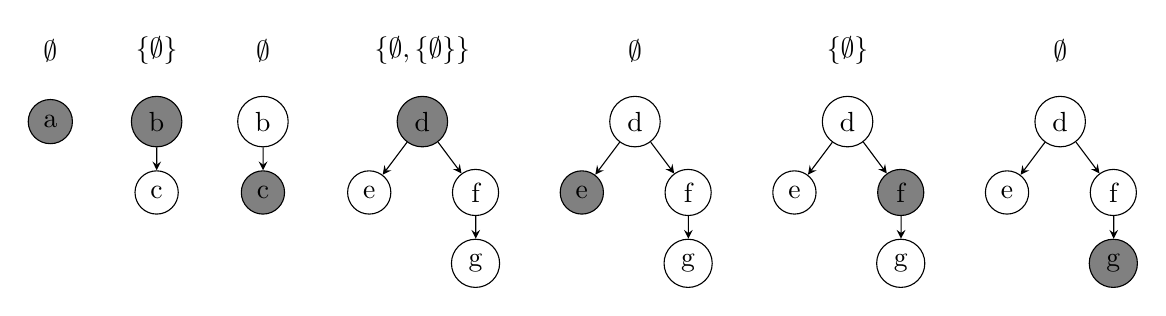
\begin{tikzpicture}[>=stealth,yscale=1.8,xscale=1.35]  

\node(h1) at (3,3.5)[text centered]{$\emptyset$};
\node(a) at (3,3)[circle,draw,text centered,fill=gray] {a};
\node(h2) at (4,3.5)[text centered]{$\{\emptyset\}$};
\node(b) at (4,3)[circle,draw,text centered,fill=gray] {b};
\node(c) at (4,2.5)[circle,draw,text centered] {c};
\node(h3) at (5,3.5)[text centered]{$\emptyset$};
\node(b1) at (5,3)[circle,draw,text centered] {b};
\node(c1) at (5,2.5)[circle,draw,text centered,fill=gray] {c};
\node(h3) at (6.5,3.5)[text centered]{$\{\emptyset,\{\emptyset\}\}$};
\node(d) at (6.5,3)[circle,draw,text centered,fill=gray] {d};
\node(e) at (6,2.5)[circle,draw,text centered] {e};
\node(f) at (7,2.5)[circle,draw,text centered] {f};
\node(g) at (7,2)[circle,draw,text centered] {g};
\node(h4) at (8.5,3.5)[text centered]{$\emptyset$};
\node(d1) at (8.5,3)[circle,draw,text centered] {d};
\node(e1) at (8,2.5)[circle,draw,text centered,fill=gray] {e};
\node(f1) at (9,2.5)[circle,draw,text centered] {f};
\node(g1) at (9,2)[circle,draw,text centered] {g};
\node(h5) at (10.5,3.5)[text centered]{$\{\emptyset\}$};
\node(d2) at (10.5,3)[circle,draw,text centered] {d};
\node(e2) at (10,2.5)[circle,draw,text centered] {e};
\node(f2) at (11,2.5)[circle,draw,text centered,fill=gray] {f};
\node(g2) at (11,2)[circle,draw,text centered] {g};
\node(h6) at (12.5,3.5)[text centered]{$\emptyset$};
\node(d3) at (12.5,3)[circle,draw,text centered] {d};
\node(e3) at (12,2.5)[circle,draw,text centered] {e};
\node(f3) at (13,2.5)[circle,draw,text centered] {f};
\node(g3) at (13,2)[circle,draw,text centered,fill=gray] {g};
                      
\draw[->] (b) -- (c); 
\draw[->] (b1) -- (c1); 
\draw[->] (d) -- (e);
\draw[->] (d) -- (f);
\draw[->] (f) -- (g);
\draw[->] (d1) -- (e1);
\draw[->] (d1) -- (f1);
\draw[->] (f1) -- (g1);
\draw[->] (d2) -- (e2);
\draw[->] (d2) -- (f2);
\draw[->] (f2) -- (g2);
\draw[->] (d3) -- (e3);
\draw[->] (d3) -- (f3);
\draw[->] (f3) -- (g3);

\end{tikzpicture}
\end{figure}

We have represented several pointed graphs where the root is indicated by the filled circle. We see that the location of the root is important as it changes the set represented by the pointed graph. In the third graph, the node $b$ has no effect because the root is $c$. \\

The operator $root$ gives the root of a pointed graph. $a/x$ replace the root of $a$ by $x$. $x~\eta_a~y$ means there is a edge in $a$ from $y$ to $x$. We have the following rewriting rules:
$$ x \ \eta_{a/z} \ y \longrightarrow x \ \eta_a \ y $$
$$ root(a/x) \longrightarrow x $$
$$ (a/x)/y \longrightarrow a/y $$

We see in the examples that some different pointed graphs can represent the same set. To characterized this, a notion of  bisimilarity, noted $\simeq$, is introduced between graphs with rewriting rule 

\begin{equation*}
\begin{split}
a \simeq b \lra~\ex r,~ &r~root(a)~root(b) \\
&\conj \ \fa x \fa x'~\fa y~(x'~\eta_a~x~\conj~r~x~y~\imp~\ex y'~(y'~\eta_b~y~\conj~r~x'~y')) \\
&\conj \ \fa y \fa y'~\fa x~(y'~\eta_b~y~\conj~r~x~y~\imp~\ex x'~(x'~\eta_a~x~\conj~r~x'~y')))
\end{split}
\end{equation*}

\begin{figure}[h]
\centering
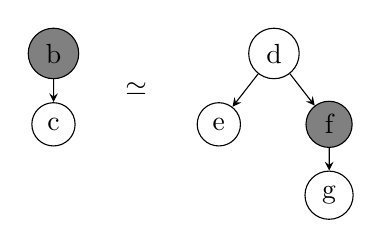
\begin{tikzpicture}[>=stealth,yscale=1.8,xscale=1.4]  

\node(b) at (5,3)[circle,draw,text centered,fill=gray] {b};
\node(c) at (5,2.5)[circle,draw,text centered] {c};
\node(d) at (7,3)[circle,draw,text centered] {d};
\node(e) at (6.5,2.5)[circle,draw,text centered] {e};
\node(f) at (7.5,2.5)[circle,draw,text centered,fill=gray] {f};
\node(g) at (7.5,2)[circle,draw,text centered] {g};
\node(h) at (5.75,2.75)[text centered]{$\simeq$};
                      
\draw[->] (b) -- (c); 
\draw[->] (d) -- (e);
\draw[->] (d) -- (f);
\draw[->] (f) -- (g);

\end{tikzpicture}
\end{figure}

In set theory, there only exists one sort: the sets. In the IZmod theory, there exists two sorts: the nodes and the pointed graphs. Therefore, there are in IZmod two constructions related to the inclusion of sets. We can take the example of $\emptyset \in \{\emptyset\}$. We can represents this inclusion in two ways, either with a relation between pointed graphs or with a relation between nodes within a same graph.

\begin{figure}[h]
\centering
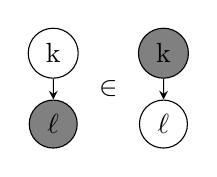
\begin{tikzpicture}[>=stealth,yscale=1.8,xscale=1.4]  

\node(d) at (6,3)[circle,draw,text centered] {k};
\node(e) at (6,2.5)[circle,draw,text centered,fill=gray] {$\ell$};
\node(k) at (6.5,2.75)[text centered]{$\in$};
\node(f) at (7,3)[circle,draw,text centered,fill=gray] {k};
\node(g) at (7,2.5)[circle,draw,text centered] {$\ell$};
                      
\draw[->] (d) -- (e);
\draw[->] (f) -- (g);

\end{tikzpicture}
\end{figure}

When in a graph we have an edge from $k$ to $\ell$, the set represented by the pointed graph with the root $\ell$ is an element of the set represented by the pointed graph with root $k$. But any pointed graph bisimilar with pointed graph with root $\ell$ also represents a set that is an element of the set represented with the pointed graph with root $k$. This leads to the definition of membership noted $\in$, with rewriting rule $a \in b \lra \ex x~(x~\eta_b~root(b)~\conj~a \simeq (b/x))$. \\

The objective of the IZmod theory is to composed pointed graphs, for instance to \textit{join} pointed graphs. The root of the new pointed graph is $o$. To guarantee that $o$ is not a node of one of the original pointed graphs, an injective function $i$ is introduced, with $i'$ its left inverse and $I$ the predicate of its image. 

$$i'(i(x)) \lra x$$
$$I(x) \lra \top$$
$$I(o) \lra \bot$$

The same method is applied to constructors $pair$, $powerset$, $etc$.

\subsection{Set Theories}

These pointed graphs permit to prove the axioms of a theory IZst that lies between Zermelo theory (Z) and Zermelo-Fraenkel theory (ZF). This theory does not contain the Replacement scheme but it contains two additional axioms: the Strong Extensionality axiom and the Transitive Closure axiom. \\

\textbf{Strong Extensionality axiom.} 
\begin{equation*}
\begin{split}
\fa x_1...\fa x_n\fa a\fa b~ &(R(a, b) \\
&\conj~\fa x\fa x'\fa y~(x' \in x \conj R(x, y) \imp \ex y'~(y' \in y \conj R(x', y'))) \\
&\conj~\fa y\fa y'\fa x~(y' \in y \conj R(x, y) \imp \ex x'~(x' \in x \conj R(x', y'))) \\
&\imp a = b) 
\end{split}
\end{equation*}

where $R(a,b)$ is a formula of free variables $x_1, ..., x_n$. \\

The hypothesis of the Strong Extensionality axiom imitates the structure of the rewriting rule of $\eta$. This can be explained with the following reasoning: in the Extensionality axiom, the hypothesis states that two sets have the same elements, so the hypothesis of the strong extensionality axiom copy the structure of one of the equivalent to the inclusion in IZmod --that is to say the constructor $\eta$. \\

\textbf{Transitive Closure axiom.} $\fa a\ex e~(a \subseteq e \conj \fa x\fa y~(x \in y \conj y \in e \imp x \in e))$ \\

The Transitive Closure axiom conveys the idea that every set is included in a transitive set. \\

The Strong Extensionality axiom can be deduced from the Foundation axiom and the Transitive Closure axiom can be derived from the Replacement Scheme.

The Strong Extensionality axiom implies the Extensionality axiom\footnote{See Section \ref{extensionality}}.

The IZmod theory is an extension of IZst set theory with an encoding of pointed graphs.

\begin{figure}[h]
\centering
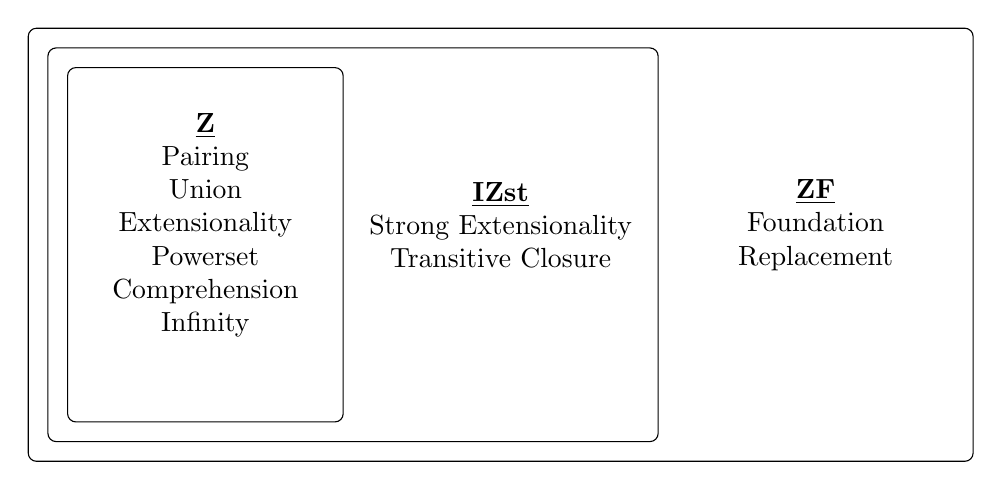
\begin{tikzpicture}[>=stealth,yscale=1,xscale=1]  

\draw[rounded corners=3pt] (0.5,0.5) rectangle (4,5);
\draw[rounded corners=3pt] (0.25,0.25) rectangle (8,5.25);
\draw[rounded corners=3pt] (0,0) rectangle (12,5.5);

\node(a) at (2.25,3)[text width=3cm,text centered] {\underline{\textbf{Z}} \\ Pairing \\ Union \\ Extensionality \\ Powerset \\ Comprehension \\ Infinity};
\node(b) at (6,3)[text width=10cm,text centered] {\underline{\textbf{IZst}} \\ Strong Extensionality \\ Transitive Closure};
\node(c) at (10,3)[text width=3cm,text centered] {\underline{\textbf{ZF}} \\ Foundation \\ Replacement};

\end{tikzpicture}
\caption{View of the different set theories}
\end{figure}


\section{The Language of Pointed Graphs}

\subsection{Sorts}

The language of the theory IZmod uses four sorts \cite[see Section 3.2]{zermodulo}. The first two are for
the pointed graphs and for the nodes of the pointed graphs.  In
\dedukti, we would need two universal quantifiers and two
existential quantifiers, one for each sort.  We rather use another
solution \cite{theoryU} that is to declare a constant $\Set$ of type
$\Type$ for codes of sorts, a function $\El$ of type $\Set \ra \Type$,
two constants $graph$ and $node$ of sort $\Set$.

\begin{lstlisting}
constant symbol graph : Set;
constant symbol node : Set;
\end{lstlisting}

The two other sorts of the theory IZmod are for classes of nodes and
for binary relations on nodes.  In \dedukti, the sort of classes is
just $\El~node \ra \El~prop$ and that of binary relations
$\El~node \ra \El~node \ra \El~prop$. To quantify on such sorts, we introduce constant $\arr $ of type
$\Set \ra \Set \ra \Set$ and rewrite rule
$$\El~(x~\arr~y) \lra (\El~x) \ra (\El~y)$$

The symbols $graph$ and $node$ are specific to the
expression of IZmod in \dedukti. In contrast the symbols $\Set$,
$\El$, $prop$, and $\arr$ are part of the standard library of 
\dedukti.

\subsection{Signature}

The signature of IZmod contains 31 symbols \cite[see Table 2]{zermodulo}. As we have replaced the
sorts for classes and relations with the \dedukti \ types
$\El~node \ra \El~prop$ and $\El~node \ra \El~node \ra \El~prop$, we do not need specific predicate symbols to apply a class to a node or a relations to two. In the same way, we do not need comprehension axioms for classes and relations. 

Similarly, the equality symbol is part of the standard library of \dedukti.

The signature is thus reduced to 26 symbols. The specific case of the comprehension symbol is treated later.

\begin{lstlisting}
symbol eta : El graph → El node → El node → El prop;
symbol root : El graph → El node;
symbol cr : El graph → El node → El graph;
constant symbol o : El node;
constant symbol O : El node;
symbol i : El node → El node;
symbol i' : El node → El node;
symbol j : El node → El node;
symbol j' : El node → El node;
symbol I : El node → El prop;
symbol J : El node → El prop;
symbol ρ : El graph → El node;
symbol ρ' : El node → El graph;
symbol Succ : El node → El node;
symbol Pred : El node → El node;
symbol Null : El node → El prop;
symbol Nat : El node → El prop;
symbol < : El node → El node → El prop;
symbol simeq : El graph → El graph → El prop;
symbol ∈ : El graph → El graph → El prop;
symbol join : El graph → El graph;
symbol pair : El graph → El graph → El graph;
symbol powerset : El graph → El graph;
symbol omega : El graph;
symbol closure : El graph → El graph;
\end{lstlisting}

\subsection{From \textit{Deduction modulo theory} to \lpcm}

Unlike \textit{Deduction modulo theory}, \lpcm ~allows quantification over propositions. \\

Thus the symbols $mem$ and $rel$ \cite[see Table 2]{zermodulo} are not needed anymore. Indeed, a class of nodes can simply be expressed as a term $P$ of type $El~node \ra El~prop$, and the fact that a node $x$ is an element of this class can be expressed as $P~x$ and not as $mem(x,P)$. In a similar way, the fact that two nodes $x$ and $y$ are related by a relation $r$ is now simply expressed with $r~x~y$.

The symbols $g_{x,y_1,...,y_n,P}$ and $g'_{x,x',y_1,...,y_n,P}$ had been created as specific constructors that allow to introduce in $mem$ a proposition $P$ by convert it into a class. These symbols are now not necessary in \dedukti ~since $mem$ is deleted. 


\subsection{Rewriting Rules}

All the other rewriting rules \cite[see Table 3]{zermodulo}, except the ones involving the symbol associated with the construction of sets by comprehension (noted $comp$), are easy to implement in \dedukti.

\begin{center}
\underline{\textbf{General}}
\end{center}

\begin{lstlisting}
rule eta (cr $a $z) $x $y ↪ eta $a $x $y;
rule root (cr $a $x) ↪ $x;
rule (cr (cr $a $x) $y) ↪ cr $a $y;
\end{lstlisting}

\begin{center}
\underline{\textbf{Relocations}}
\end{center}

\begin{lstlisting}
rule i' (i $x) ↪ $x;
rule j' (j $x) ↪ $x;
rule ρ' (ρ $x) ↪ $x;
rule I (i $x) ↪ ⊤;
rule J (j $x) ↪ ⊤;
rule I (j $x) ↪ ⊥;
rule J (i $x) ↪ ⊥;
rule I (o) ↪ ⊥;
rule J (o) ↪ ⊥;

rule Pred (Succ $x) ↪ $x ;
rule Null O ↪ ⊤;
rule Nat O ↪ ⊤;
rule Null (Succ $x) ↪ ⊥;
rule Nat (Succ $x) ↪ Nat $x;

rule $x < O ↪ ⊥;
rule $x < (Succ $y) ↪ ($x < $y) ∨ ($x = $y);
\end{lstlisting}

\begin{center}
\underline{\textbf{Equality and Membership}}
\end{center}

\begin{lstlisting}
rule $a simeq $b ↪ `∃ r : El (node arrow (node arrow prop)), 
    r (root $a) (root $b)
    ∧ (`∀ x, `∀ x', `∀ y, 
        eta $a x' x ∧ r x y
            ⇒ `∃ y', eta $b y' y ∧ r x' y')
    ∧ (`∀ y, `∀ y', `∀ x, 
        eta $b y' y ∧ r x y
            ⇒ `∃ x', eta $a x' x ∧ r x' y');

rule $a ∈ $b ↪ `∃ x, ((eta $b x (root $b)) ∧ ($a simeq cr $b x));
\end{lstlisting}

\begin{center}
\underline{\textbf{Constructions}}
\end{center}

\begin{lstlisting}
rule eta (join $a) $x $x' ↪ 
	(`∃ y, `∃ y', ($x = i y) ∧ ($x' = i y') ∧ eta $a y y')
    ∨ (`∃ y, `∃ z, ($x = i y) 
    	∧ ($x' = o) 
    	∧ eta $a y z 
    	∧ eta $a z (root $a));

rule eta (pair $a $b) $x $x' ↪ 
	(`∃ y, `∃ y', (($x = i y) ∧ ($x' = i y') ∧ eta $a y y'))
    ∨ (`∃ y, `∃ y', ($x = j y) ∧ ($x' = j y') ∧ eta $b y y')
    ∨ (($x = i (root $a)) ∧ ($x' = o))
    ∨ (($x = j (root $b)) ∧ ($x' = o));

rule eta (powerset $a) $x $x' ↪ 
	(`∃ y, `∃ y', ($x = i y) ∧ ($x' = i y') ∧ eta $a y y')
    ∨ (`∃ y, `∃ c, ($x = i y) 
    	∧ ($x' = j (ρ c)) 
    	∧ (eta $a y (root $a)) 
    	∧ ((cr $a y) ∈ c))
    ∨ (`∃ c, ($x = j (ρ c)) ∧ ($x' = o));

symbol omega : El graph;
rule eta omega $x $x' ↪ 
	(`∃ y, `∃ y', ($x = i y) ∧ ($x' = i y') ∧ (y < y'))
    ∨ (`∃ y, ($x = i y) ∧ ($x' = o) ∧ Nat y);

symbol closure : El graph → El graph;
rule eta (closure $a) $x $x' ↪ 
	(`∃ y, `∃ y', (($x = i y) ∧ ($x' = i y') ∧ eta $a y y'))
	∨ (`∃ y, ($x = i y) 
        ∧ ($x' = o)
        ∧ (`∀ c : El (node arrow prop), 
                ((`∀ z, eta $a z (root $a) ⇒ c z)
                ∧ (`∀ z, `∀ z', (eta $a z z') ∧ (c z') ⇒ (c z)))
            ⇒ c y));
            
rule root (join $a) ↪ o;
rule root (pair $a $b) ↪ o;
rule root (powerset $a) ↪ o;
rule root omega ↪ o;
rule root (closure $a) ↪ o;

\end{lstlisting}

The pointed graph \texttt{omega} represents the set of Von Neumann ordinals \cite[see Table 2]{zermodulo53}. Indeed, the informal presentation of the representation of sets by pointed graphs given in \ref{informal} corresponds to Von Neumann ordinals. The rewriting rule of \texttt{eta omega x x'} states that in \texttt{omega} the edges represents the order relation $<$ and that there is an edge from every natural number to the root of \texttt{omega}.


\section{The Language of Formulas}

A key point in the original formulation of the theory is that the lemmas in which the $comp$ symbol --enabling to construct a set by comprehension-- is used are only valid for a subset of formulas \cite[see Table 5]{zermodulo}. The formulas need to have all of its quantifiers of sort $El~graph$ and can only use the language $\in$, $\simeq$ and the classic logical connectives. Taking this restriction into account was the main challenge of this implementation.

Thus we need to introduce a set to characterize the validity domain of such lemmas.

\subsection{Formulas}

In order to achieve this goal, we define the constant $formula$ of type $\Set$ and the logical connectives related to this constant.

\begin{lstlisting}
constant symbol formula : Set;
constant symbol eqF : El nat → El nat → El formula;
constant symbol inF : El nat → El nat → El formula;
constant symbol andF : El formula → El formula → El formula;
constant symbol orF : El formula → El formula → El formula;
constant symbol allF : El nat → El formula → El formula;
constant symbol exF : El nat → El formula → El formula;
constant symbol impF : El formula → El formula → El formula;
constant symbol fF : El formula;
constant symbol tF : El formula;
\end{lstlisting}

Then we are able to define an induction over formulas, using the language $\in$, $\simeq$ and the classic logical connectives.

\begin{lstlisting}
constant symbol recF : Π (P : El formula → Prop), 
π(`∀ x, `∀ y, P (eqF x y))
→ π(`∀ x, `∀  y, P (inF x y))
→ π(`∀ f, `∀ g, (P f ∧ P g) ⇒ (P (andF f g)))
→ π(`∀ f, `∀ g, (P f ∧ P g) ⇒ (P (orF f g)))
→ π(`∀ f, `∀ g, (P f ∧ P g) ⇒ (P (impF f g)))
→ π(`∀ f, (P f) ⇒ (`∀ x, P (allF x f)))
→ π(`∀ f, (P f) ⇒ (`∀ x, P (exF x f)))
→ π(P tF)
→ π(P fF)
→ π(`∀ f, P f);
\end{lstlisting}

\subsection{Interpretation}

The next step is to interpret an object of type $formula$ into $Prop$. We introduce the constant $interpretation$ which receives a valuation of type $\El \ nat \ \ra \ \El~graph$ and a formula of type $\El \ formula$ and return a $\El~prop$.

\begin{lstlisting}
symbol interpretation : (El nat → El graph) → El formula → El prop;
\end{lstlisting} 

We need to have a tool to update a valuation when we assign a variable. To do so, we introduce the constant $update$ of type $(\El \ nat \ra \El~graph) \ra \El \ nat \ra \El~graph \ra (\El \ nat \ra \El~graph)$ which takes as arguments a valuation $\sigma$, a natural number $x$ and a graph $a$ and returns a new valuation $(update \ \sigma \ x \ a)$ that substitutes $x$ by $a$ and acts like $\sigma$ for the other natural numbers.

To write a rewriting rule upon $update$, we need to be able to check if we apply $(update \ \sigma \ x \ a)$ to $y = x$ (which is substituted by $a$) or to $y \neq x$ (which is substituted by $\sigma \ y$.

We define the symbol $update1$ of type $(\El \ nat \ \ra \ \El~graph) \ \ra \ \El \ nat \ \ra \ \El~graph \ \ra \ \El \ nat \ \ra \ (\El \ nat \ \ra \ \El~graph)$.

The technique we use to rewrite $(update \ \sigma \ x \ a) \ y $ is the following: 

\begin{itemize}
\item We keep in memory $y$ in the new argument $z$ of $update1$
$$(update \ \sigma \ x \ a) \ y \ \lra \ update1 \ \sigma \ x \ a \ y \ y$$
\item We decrement $x$ and $y$ until one of them equals zero
$$update1 \ \sigma \ (s \ x) \ a \ (s \ y) \ z \ \lra \ update1 \ \sigma \ x \ a \ y \ z$$
\item If both are equal to zero, then $x$ and $y$ are equal and we return $a$. 
$$ update1 \ \sigma \ zero \ a \ zero \ z \ \lra \ a$$
If only one equals zero, then they are different and we return $\sigma \ z$.
$$update1 \ \sigma \ zero \ a \ (s \ y) \ z \ \lra \ \sigma \ z$$
$$update1 \ \sigma \ (s \ x) \ a \ zero \ z \ \lra \ \sigma \ z$$
\end{itemize}

Now we have all the tools to define the rewriting rules of the interpretation of formulas:

$$interpretation \ \sigma \ (eqF \ x \ y) \lra (\sigma \ x) \ \simeq \ (\sigma \ y)$$
$$interpretation \ \sigma \ (inF \ x \ y) \lra (\sigma \ x) \ \in \ (\sigma \ y)$$
$$interpretation \ \sigma \ (andF \ f \ g) \lra (interpretation \ \sigma \ f) \conj (interpretation \ \sigma \ g)$$
$$interpretation \ \sigma \ (orF \ f \ g) \lra (interpretation \ \sigma \ f) \disj  (interpretation \sigma \ g)$$
$$interpretation \ \sigma \ (impF \ f \ g) \lra (interpretation \ \sigma \ f) \imp (interpretation \ \sigma \ g)$$
$$interpretation \ \sigma \ (allF \ x \ f) \ \lra \ \fa a, interpretation \ (update \ \sigma \ x \ a) \ f$$
$$interpretation \ \sigma \ (exF \ x \ f) \ \lra \ \ex a, interpretation \ (update \ \sigma \ x \ a) \ f$$
$$interpretation \ \sigma \ fF \lra \blbot$$
$$interpretation \ \sigma \ tF \lra \bltop$$

\subsection{Results concerning Valuation}

Thanks to the introduction of $interpretation$, we can deduce five theorems. \\

The first theorem is used to simplify the terms when updating a valuation.

\begin{theorem}
$\fa \sigma \fa x \fa y \fa z \fa a ~((x = y \ \imp \ update1 \ \sigma \ x \ a \ y \ z \ \simeq \ a) \ \conj \ (\blneg \ x = y \ \imp \ update1 \ \sigma \ x \ a \ y \ z \ \simeq \ \sigma \ z))$
\end{theorem}

\begin{proof}
The first term of the conjunction is proved by simple recurrence over natural numbers. The second term of the conjunction is proved by double recurrence. $\square$
\end{proof}

The second theorem conveys the idea that if two graphs are bisimilar then it is identical to update a valuation by either of theses two graphs.

\begin{theorem}
$\fa \sigma \fa x \fa a \fa b ~(a \ \simeq \ b \ \imp \ \fa y ~(update \ \sigma \ x \ a \ y \ \simeq \ update \ \sigma \ x \ b \ y))$
\end{theorem}

\begin{theorem}
$\fa \sigma \fa x \fa y \fa a \fa b \fa c ~(a \ \simeq \ b \ \imp \ \fa z~ (update \ (update \ \sigma \ x \ a) \ y \ c \ z \ \simeq \ update \  (update \ \sigma \ x \ b) \ y \ c \ z))$
\end{theorem}

The fourth theorem states that if two valuations are equal they keep being equal after an update.

\begin{theorem}
$\fa \sigma \fa \sigma' \fa x \fa c~ ((\fa y~ (\sigma \ y \ \simeq \ \sigma' \ y)) \ \imp \ \fa z~ (update \ \sigma \ x \ c \ z \ \simeq \ update \ \sigma' \ x \ c \ z))$
\end{theorem}

\begin{theorem}
$\fa f \fa \sigma \fa \sigma' ~((interpretation \ \sigma \ f \ \conj \ \fa x ~(\sigma \ x \ \simeq \ \sigma' \ x)) \ \imp \ interpretation \ \sigma' \ f)$
\end{theorem}

\begin{proof}
The fifth theorem is proved by induction over formulas. $\square$
\end{proof}

\subsection{Comprehension, Empty Set and Inductive Set}

Henceforth, we are able to define in \dedukti
$$comp : \El~graph \ra (\El \ nat \ \ra \ \El~graph) \  \ra \El \ formula \ra \ \El~graph$$

and its rewriting rules

\begin{lstlisting}
rule eta (comp $a $σ $f) $x $x' ↪ 
	(`∃ y, `∃ y', (($x = i y) ∧ ($x' = i y') ∧ eta $a y y')) 
	∨ (`∃ y, ($x = i y) ∧ ($x' = o) ∧ (eta $a y (root $a))
	∧ (interpretation (update $σ zero (cr $a y)) $f));
rule root (comp $a $σ $f) ↪ o;
\end{lstlisting}

When it comes to the symbol related to the Infinity section of \cite[see Section 2.1]{zermodulo}, we implement $empty\_set$ of type $\El~graph$ and $Ind$ of type $\El~graph \ \ra \ \El~prop$.

To define the empty set, we use $comp$ with the formula $fF$:
\begin{lstlisting}
rule empty_set ↪ comp omega (λ _, empty_set) fF;
rule root empty_set ↪ o;
\end{lstlisting}

Then we implement

\begin{lstlisting}
rule Ind $c ↪ (empty_set ∈ $c) 
∧ (`∀ a, (a ∈ $c) ⇒ ((join (pair a (pair a a))) ∈ $c));
\end{lstlisting}


\section{Lemmas}

A first result on the original formulation of the theory was to prove that the axioms of IZst are theorems in IZmod. This required 53 lemmas that were \textit{informally} proved in \cite[see Tables 4 and 5]{zermodulo} and that we prove \textit{formally} in this paper.

Some of these proofs just follow the informal ones. Some others require the use of the type of formula and its embedding into propositions. 

The first lemma $x=x$ does not need to be implemented since it is already part of the standard library of \dedukti \ under the name \texttt{refl} (which is polymorphic).

The second lemma is already a consequence of the rewriting rule of the polymorphic $=$ implemented in the standard library of \dedukti: 
\begin{lstlisting}
constant symbol = [s] : El s → El s → El prop;
notation = infix 4;
rule π (@= $s $x $y) ↪ Π (P : El $s → El prop), π(P $x) → π(P $y);
\end{lstlisting}

All the other lemmas of IZmod except the ones where $comp$ is involved are proved using the blueprint in \cite[see Proposition 1]{zermodulo53}. The complete proofs can be found in \url{https://github.com/Deducteam/dedukti_set_theory/}.

\subsection{An Example of Proof}

To show the way lemmas are proved in \dedukti ~we will take the example of lemma 30 and comment its proof. This lemma states that $$ a \in b \conj a \simeq c \imp c \in b $$

\begin{proof}
We first assume graphs $a$, $b$ and $c$ and $H$ the proof of $ a \in b \conj a \simeq c $. $a \in b$ rewrites to $\ex x~(x~\eta_b~root~b \conj a \simeq (b/x))$. 

We make appear $x$ and $Hx$ the proof $x~\eta_b~root~b \conj a \simeq (b/x)$. 

As the goal is to prove $c \in b$, that is to say $\ex y~(y~\eta_b~root~b \conj c \simeq (b/y))$, we need to find a suitable $y$. We take $x$ and now have two goals: $y~\eta_b~root~b$ and $c \simeq (b/y)$. 

The first one is proved by applying the left part of $Hx$. 

The second one is obtained by applying lemma 5 to $c$, $a$ and $b/x$. To apply lemma 5, we need to prove $c \simeq a \imp a \simeq b/x$. $c \simeq a$ is proved applying reflexivity to $a \simeq c$ (i.e. applying lemma 4 to $a$, $c$ and the right part of $H$). $a \simeq b/x$ derives from the right part of $Hx$. $\square$
\end{proof}

This proof is written in \dedukti ~with the following code: 

\begin{lstlisting}
opaque symbol lemma30 : π(`∀ a, `∀ b, `∀ c, 
	((a ∈ b) ∧ (a simeq c)) ⇒ (c ∈ b))
≔ begin
assume a b c H;
refine ex_e node _ (and_el _ _ H) _ _;
assume x Hx;
refine ex_i node x _ _;
refine and_i _ _ _ _
{refine and_el _ _ Hx}
{refine lemma5 c a (cr b x) 
	(and_i _ _ (lemma4 a c (and_er _ _ H)) (and_er _ _ Hx))}
end;
\end{lstlisting}

\subsection{Lemmas involving Formulas}

Now that the language of formulas have been designed along with the implementation of the $comp$ symbol, lemma 32 can be implemented.

$$(P(z \leftarrow a) \conj a \simeq b) \imp P(z \leftarrow b)$$

We implement it thanks to the $interpretation$ symbol. The valuation $update~\sigma~z~a$ represents the assignment of variable $z \leftarrow a$.

\begin{lstlisting}
opaque symbol lemma32 : Π (z : El nat), Π (f : El formula), 
	π(`∀ a, `∀ b, (`∀ σ : (El nat → El graph),
	((interpretation (update σ z a) f) ∧ (a simeq b)) 
	⇒ (interpretation (update σ z b) f)))
\end{lstlisting}

The proof of this \texttt{opaque symbol} is done by induction over formulas: each case is proved easily, using the lemmas that have already been checked by \dedukti. \\

Lemma 41 is implemented similarly:

\begin{lstlisting}
opaque symbol lemma41 : Π (x y : El nat), Π (f : El formula), 
	Π (c d : El graph), π(`∀ σ : (El nat → El graph), 
	((interpretation (update (update σ x c) y d) f)
	∧ (`∀ a, `∀ a', `∀ b, 
		((a' ∈ a) 
		∧ (interpretation (update (update σ x a) y b) f)) 
		⇒ (`∃ b', ((b' ∈ b) 
			∧ (interpretation (update (update σ x a') y b') f))))
	∧ (`∀ b, `∀ b', `∀ a, 
		((b' ∈ b) 
		∧ (interpretation (update (update σ x a) y b) f)) 
		⇒ (`∃ a', ((a' ∈ a) 
			∧ (interpretation (update (update σ x a') y b') f))))) 
	⇒ (c simeq d))
\end{lstlisting}

\subsection{Weak Extensionnality}

\label{extensionality}

We notice in \cite{zermodulo53} the use of weak extensionality (simply called extensionality) to prove lemmas 44, 47 and 48. We want to deduce weak extensionality from strong extensionality (i.e. lemma 41). \\

\textbf{Weak extensionality.} $\fa c\fa d~ (\fa z~ (z \in c \Leftrightarrow z \in d) \imp c \simeq d)$ \\

We follow the blueprint given by G. Dowek and A. Miquel \cite[see Proposition 1]{zermodulo} : we use the strong extensionality axiom where $R(x,y)$ is $(x \simeq c~\conj~y \simeq d)~\disj~x \simeq y$. \\

\begin{proof}
We want to prove that $\fa c\fa d~(\fa z~ (z \in c \Leftrightarrow z \in d) \imp c \simeq d)$. We assume that $\fa z~ (z \in c \Leftrightarrow z \in d)$. We want to apply strong extensionality to deduce $c \simeq d$. To do so, we need to prove the three terms of the hypothesis of strong extensionality.

$(c \simeq c~\conj~d \simeq d)~\disj~c \simeq d$ is a tautology.

We want to prove that $\fa a\fa a'\fa b~(a' \in a~\conj~((a \simeq c~\conj~b \simeq d)~\disj~a \simeq b) \imp (\ex b'~ (b' \in b~\conj~((a' \simeq c~\conj~b' \simeq d)~\disj~a' \simeq b'))$. We assume $(a' \in a~\conj~((a \simeq c~\conj~b \simeq d)~\disj~a \simeq b)$. If $(a \simeq c~\conj~b \simeq d)$, then we choose $b' \simeq a'$. We have $b' \in a$ because $a' \in a$. Yet, $a \simeq c$, $c \simeq d$ and $d \simeq b$. Then $b' \in b$. If $a \simeq b$, we choose $b' \simeq a'$. We have $b' \in a$ because $a' \in a$. Yet, $a \simeq b$. Thus $b' \in b$.

We proceed similarly for the third term. $\square$
\end{proof}

We implement this theorem in \dedukti:

\begin{lstlisting}
opaque symbol lemmaHypExt : Π (c d : Graph), 
	π((`∀ z, (z ∈ c) ⇔ (z ∈ d)) ⇒ 
	((((c simeq c) ∧ (d simeq d)) ∨ (c simeq d))
	∧ (`∀ a, `∀ a', `∀ b, 
		((a' ∈ a) ∧ (((a simeq c) ∧ (b simeq d)) ∨ (a simeq b))) 
		⇒ (`∃ b', ((b' ∈ b) 
		∧ (((a' simeq c) ∧ (b' simeq d)) ∨ (a' simeq b')))))
	∧ (`∀ b, `∀ b', `∀ a, 
		((b' ∈ b) ∧ (((a simeq c) ∧ (b simeq d)) ∨ (a simeq b)))
		 ⇒ (`∃ a', ((a' ∈ a) 
	 	∧ (((a' simeq c) ∧ (b' simeq d)) ∨ (a' simeq b')))))))
\end{lstlisting}

To prove $weak \ extensionality$, we assume graphs $c$ and $d$, and $H$ the hypothesis $\fa z~ (z \in c) \Leftrightarrow (z \in d)$. Then we apply lemma 41 to:

\begin{itemize}
\item natural numbers $zero$ and $one$
\item the formula $(orF~(andF~(eqF~zero~two)~(eqF~one~three))~(eqF~zero~one))$
\item graphs $c$ and $d$
\item the valuation $(update~(update~(\lambda \_, empty\_set)~two~c)~three~d)$ 
\item the proof of the left hand term $lemmaHypExt~c~d~H$.
\end{itemize}

Indeed, in the formula $$(orF~(andF~(eqF~zero~two)~(eqF~one~three))~(eqF~zero~one))$$ $zero$ and $one$ will be interpreted by $c$ and $d$ thanks to lemma 41 and $two$ will be interpreted by $c$ and $three$ by $d$ thanks the valuation $$(update~(update~(\lambda \_, empty\_set)~two~c)~three~d)$$ The proposition obtained corresponds to the proposition in lemmaHypExt.


\begin{lstlisting}
opaque symbol lemmaExt : Π (c d : El graph), 
	π((`∀ x, (x ∈ c) ⇔ (x ∈ d)) ⇒ (c simeq d))
≔ begin
assume c d H;
refine lemma41 zero one 
	(orF (andF (eqF zero two) (eqF one three)) (eqF zero one)) 
	c d (update (update (λ _, empty_set) two c) three d) 
	(lemmaHypExt c d H)
end;
\end{lstlisting}

\subsection{The Axioms of IZst Theory}

We have now encoded in \dedukti ~all the axioms of IZst set theory: the strong extensionality axiom corresponds to lemma 41, the axiom of the union is implemented by lemma 42, the pairing axiom corresponds to lemma 43, the axiom of the power set is encoded by lemma 44, the comprehension scheme is implemented by lemma 45, the axiom of infinity corresponds to lemma 51 and the transitive closure axiom is encoded by lemmas 52 and 53.


\section{Conclusion}

We have implemented in \dedukti ~a version of set theory -- IZst -- that corresponds to Zermelo set theory, with the Strong Extensionality axiom and the Transitive Closure axiom. To do so, we have adapted the work by G. Dowek and A. Miquel \cite{zermodulo} from \textit{Deduction modulo theory} to \lpcm ~and have encoded sets with a structure of pointed graphs of the IZmod theory. We have \textit{formally} written all the proofs of the lemmas allowing us to implement set theory in \dedukti.

To define and prove the lemmas corresponding to the Comprehension axiom, we have developed a language of formulas, along with operators \textit{interpretation} and \textit{update}. In particular, the language of formulas allows us to prove that the Extensionality axiom derives from the Strong Extensionality axiom.

Historically, the encoding of sets by pointed graphs had been designed to enjoy the normalization property. IZmod expressed in \textit{Deduction modulo theory} does so, but the case of our implementation in \lpcm ~remains to be investigated.

The implementation of IZmod theory represents a significant corpus of formal proofs in \textsc{Lambdapi}.

\newpage
\section*{Annex}

\begin{center}
\begin{tabular}{|c|c||c|c|}
\hline Lemma & Number of lines in the proof & Lemma & Number of lines in the proof \\
\hline 3 & 26 & 29 & 17 \\
\hline 4 & 14 & 30 & 10 \\
\hline 5 & 37 & 31 & 12 \\
\hline 6 & 33 & 32 & 49 \\
\hline 7 & 12 & 33 & 33 \\
\hline 8 & 5 & 34 & 33 \\
\hline 9 & 12 & 35 & 9 \\
\hline 10 & 12 & 36 & 9 \\
\hline 11 & 5 & 37 & 9 \\
\hline 12 & 5 & 38 & 9 \\
\hline 13 & 5 & 39 & 9 \\
\hline 14 & 37 & 40 & 9 \\
\hline 15 & 40 & 41 & 42 \\
\hline 16 & 48 & Weak extensionality & 47 \\
\hline 17 & 48 & 42 & 49 \\
\hline 18 & 38 & 43 & 39 \\
\hline 19 & 44 & 44 & 133 \\
\hline 20 & 90 & 45 & 46 \\
\hline 21 & 34 & 46 & 11 \\
\hline 22 & 35 & 47 & 18 \\
\hline 23 & 34 & 48 & 165 \\
\hline 24 & 38 & 49 & 11 \\
\hline 25 & 31 & 50 & 23 \\
\hline 26 & 38 & 51 & 6 \\
\hline 27 & 29 & 52 & 17 \\
\hline 28 & 33 & 53 & 31 \\
\hline
\end{tabular}
\end{center}




%\nocite{*}
\bibliographystyle{eptcs}
\bibliography{biblio}
\end{document}
